\chapter{Gravitational wave antennae}
\label{ch:ifo}
This chapter covers some of the essentials of laser interferometer gravitational wave antennae. %NL%
For futher information, the author suggests the incredible introductory treatment by \citet{saulson1994fundamentals}. %NL%
Some great resources on the details of the LIGO experiment are contained in the theses of \citet{ranathesis} and \citet{stefanthesis}, and more recently \citet{FrickeThesis}, \citet{dooleythesis} and \citet{kisselthesis}.
\section{Experimental efforts to detect gravitational waves}
In 1960, Joseph Weber made the suggestion that an aluminum bar could be used as a gravitational wave antenna \cite{bar1}. %NL%
The idea being that as a burst of gravitational wave passes, it would induce a strain in the bar and excite the resonant mechanical modes of the bar. %NL%
For reasons detailed elsewhere\cite{bar2,bar3}, the scientific community was never able to verify Weber's subsequent claims of detection\cite{bar4} although various theories\cite{bar5,bar6} were developed to explain the enormous apparent flux of gravitational wave energy.

In the subsequent years following Weber’s pioneering work, resonant bar detectors have improved greatly. %NL%
Modern bar detectors are cryogenically cooled, have much improved seismic isolation and make use of SQUIDs to readout the signal \cite{bar7}.

Using light waves to measure gravitational pertubations was first pointed out by Pirani in 1956 \cite{ifo1}. %NL%
It was only until 1971 that an early prototype interferometer was built in Malibu using an audio cassete recorder for data acquisition \cite{ifo2}. %NL%
Shortly after that, a study done at MIT by R. %NL%
Weiss identified almost all noise sources relevant for a kilometer length scale interferometer \cite{ifo3}. %NL%
It is these broadband laser interferometer based gravitational wave antennae which provide the most compelling chance to directly measure these elusive waves.

In recent years, kilometer scale interferometers have been constructed and operated with the purpose of searching for gravitational waves. %NL%
These are the American LIGO interferometers \cite{LIGO}, the German-English GEO600 interferometer \cite{GEO600}, and the Italian-French Virgo interferometer \cite{Virgo}.

\section{Measurement of optical phase}
In Chapter \ref{ch:gws} we introduced the idea that the waveform of a passing gravitational wave is imprinted on the phase of photons. %NL%
The frequency of ocillation of a laser with a wavelength of 1.064$\upmu$m is 2.8$\times 10^{14}$Hz. %NL%
There is no technology, currently concieved, with which one can directly measure the phase of electromagnetic waves at optical frequencies. %NL%
One may, however, convert the change of phase of the electromagnetic wave into a change of amplitude by means of the phenomenon of interference. %NL%
This is acheived by superposing two electromagnetic waves and measuring the power of the resulting wave, which is straightforward with the use of a photodetector (PD). %NL%


A device which exploits interference to measure phase changes of light is refered to as an \emph{interferometer}. %NL%
Modern interferometers use one or multiple lasers as the source of light. %NL%
Laser light is very well equipped for interferometry, is highly phase coherent compared to other light sources and a laser beam can often approach the minimum beam divergence physically allowed. %NL%
Types of interferometers include: Fabry-Perot, Michelson, Mach-Zehnder etc.

\section{Resonant optical cavity}
A resonant cavity, sometimes refered to as a Fabry-Perot (FP) cavity, is constructed with two partially transmitting mirrors placed in series. %NL%
When light is incident on the front, or input, mirror, some of that light is transmitted into the cavity. %NL%
As a steady state is approached, the light already in the cavity may interfere with new light which is being pumped through the input mirror. %NL%
When the circulating field is in phase with the incident pumping field, \emph{resonance} occurs. %NL%
Assuming plane waves and a linear cavity, this happens when the length is equal to an integer number of half-wavelengths of the light \cite{Siegman}.

\begin{figure}
  \begin{center}
  \leavevmode
  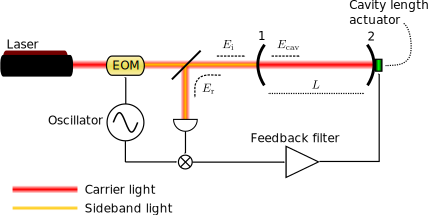
\includegraphics{figs-ifo/resonantcav.pdf}
  \end{center}
  \caption[Diagram of a resonant cavity and control system]{Diagram of a resonant cavity and control system. In this representation, the cavity is held on resonance by feeding back to the position of the end mirror. Alternatively, resonance can be acheived by feeding back to the laser frequency, causing the laser wavelength to follow the length of the cavity.}
  \label{fig:resonantcav}
\end{figure}

We may consider the interference condition after steady state has been acheived as there being a intracavity field, $E_{\rm{cav}}$, which is made up of some of the input light, $E_{\rm i}$ which has been transmitted, and some cavity light which has made a round trip path through the cavity. %NL%
The arrangement of the fields may be seen in Figure \ref{fig:resonantcav}.
\begin{equation}
E_{\rm{cav}}=t_1 E_{\rm i} + r_1 r_2 e^{i 2 k L} E_{\rm{cav}},
\end{equation}
where $r_j$ and $t_j$ are the amplitude reflection and transmission coefficients of the cavity mirrors, for $j=\{1,2\}$ with 1 being the label of the input mirror, and 2 being the label of the end mirror. %NL%
This allows us to solve for the intra-cavity field
\begin{equation}
E_{\rm{cav}}=\frac{t_1}{1 - r_1 r_2 e^{i 2 k L}} E_{\rm i}.
\end{equation}
The reflected field is
\begin{equation}
E_{\rm{r}}=-r_1 E_{\rm i} + t_1r_2 e^{i 2 k L} E_{\rm{cav}}=\frac{-r_1+(r_1^2+t_1^2)e^{i2kL}r_2}{1-r_1r_2e^{i2kL}}E_{\rm i}.
\end{equation}
Assuming no loss of the input mirror ($r_1^2+t_1^2=1$), the cavity field contains a factor of $r_2-r_1$ on resonance. %NL%
Thus the sign of the reflected field on resonance depends on the relative magnitudes of the reflectivities of the cavity mirrors. %NL%
In fact, when the reflectivities are equal, one has perfect impedence mathcing and no field is reflected. %NL%
The case of $r_2>r_1$ is known as overcoupled, and the reflected field changes sign when passing through resonance. %NL%
When $r_2<r_1$, there is no sign change, and this is known as undercoupled. %NL%
The case when no field is reflected ($r_2=r_1$) is known as critically coupled. %NL%
The LIGO arm cavities (Section \ref{sec:armcav}) are an example of strongly overcoupled cavities, while the output mode cleaner (Chapter \ref{ch:omc}) is a critically coupled cavity. %NL%
Undercoupled cavities are more rare because the majority of the light does not penetrate the cavity and thus does not provide a very sensative measurement.

The phase change on reflection is enhanced relative to the phase change inside the cavity. %NL%
For a change of the intracavity phase $\phi = k L$, the phase of the reflected field will change as
\begin{equation}
\phi_r=2\tan^{-1}\left(\frac{2\mathcal{F}}{\pi}\phi\right),
\end{equation}
where $\mathcal{F}$ is known as the \emph{cavity finesse} and has the approximate value $\mathcal{F}\approx \pi\frac{\sqrt{r_1r_2}}{1-r_1r_2}$ where the approximation is valid for $\{r_1,r_2\}\approx 1$. %NL%
For large values of the finesse, the phase of the reflected field has a steep variation compared to the intracavity phase. %NL%
A very typical cavity may have a value of the finesse which is a few hundred. %NL%
Colloquially this can be viewed in the particle picture of light that the photons bounce around in the cavity many times before exiting and thus experience an accumulated phase gain many times that of a single round trip.

%\infobox{Coupling conditoin of a resonant cavity}{
%\begin{wrapfigure}{r}{.4\textwidth}
%\begin{tabular}{|p{5cm}|}
%Coupling condition of a resonant cavity\\
%\begin{itemize}
%\item $r_1<r_2$: Overcoupled, reflected field changes sign on resonance.
%\item $r_1>r_2$: Undercoupled, no sign change on resonance.
%\item $r_1=r_2$: Critically coupled, no field reflected on resonance.
%\end{itemize}
%\end{tabular}
%\end{wrapfigure}
%}
\section{Pound-Drever-Hall reflection locking}
Pound-Drever-Hall (PDH) reflection locking is a powerful technique by which the resonance condition of a laser incident on an optical cavity may be controlled by use of a feedback control system \cite{PDH}. %NL%
In this control system, the error signal is a measurement of the detuning of the laser light from resonance. %NL%
In the case of a fixed length cavity, this may be understood as a measurement of the fluctuations in the laser wavelength. %NL%
We are instead concerned with a very stable laser source and a cavity which may change length due to external influences.\footnote{A gravitational wave changes the phase accumulated in the cavity, which is essentially interchangable with the optical path length of the cavity.} In this case, the error signal is better understood as a measurement of the length changes of the cavity.

As was shown in the previous section, the phase shift of the beam reflected from the resonant cavity is enhanced for fields resonant in the cavity. %NL%
However, for fields not resonant in the cavity, there is nearly no phase shift of the reflected beam. %NL%
The PDH sensing technique exploits this fact by contructing an input beam with frequency components that are both resonant and non-resonant. %NL%
By doing a relative phase measurement of the reflected fields, one may determine length changes of the cavity.

Creation of the input beam is done by sending the beam through an optical modulator. %NL%
This usually comes in the form of an \emph{electro optic modulator} (EOM), which is an optical device that has a electronically variable optical path length. %NL%
Applying a periodic electronic signal, usually at radio frequencies (RF), will induce a periodic phase modulation of the laser beam. %NL%
As will be discussed in Section \ref{sec:freqspace}, the primary result of this phase modulation is to impose new optical fields separated in frequency from the original field by the RF modulation frequency. %NL%
These new fields are usually refered to as \emph{phase modulated sidebands}, the central frequency component is refered to as the \emph{carrier}. %NL%
Figure \ref{fig:resonantcav} shows a typical arrangement of a PDH control system. %NL%
The modulation frequency is chosen such that the sidebands are not resonant in the cavity, and thus do not experience a phase shift when the cavity changes length. %NL%
Comparison of the constant sideband phase with the resonating carrier phase through interferometry yields a very sensitive cavity length measurement. %NL%


Because the modulator is varying the phase of the laser field, ideally there is no associated amplitude modulation. %NL%
Mathematically this is represented by the phase sidebands having an imaginary amplitude when compared to the carrier, they have a 90\degrees{} relative angle in the complex phasor plane. %NL%
The arm-cavities are strongly overcoupled, thus when the carrier is exactly centered on resonance, the reflected field experiences a 180\degrees{} phase shift. %NL%
Thus the phase sidebands are still phase sidebands. %NL%
When the carrier is slightly detuned from resonance, the relative angle between the carrier and sidebands changes and what were once pure phase sidebands now have some amount of amplitude component. %NL%
Thus the power in the reflected beam now experiences a modulation. %NL%
Demodulating the power recorded by a photodetector in reflection will provide the desired length error signal.

\section{The Michelson interferometer}
The pre-stabilized laser and input optics systems provide the LIGO interferometers with an extremely stable light source with which to measure phase pertubations. %NL%
To provide a phase sensitivity necessary to detect gravitational waves it will be necessary to play a few tricks to hide our gravitational wave readout system from the noise still present on the input laser.

\begin{figure}
  \begin{center}
  \leavevmode
  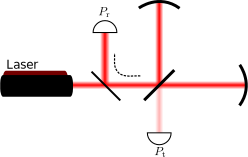
\includegraphics{figs-ifo/michelson.pdf}
  \end{center}
  \caption[Diagram of a Michelson interferometer.]{Diagram of Michelson interferometer. Photodetectors are arranged to measure the transmitted power, $P_{\rm t}$, and the reflected power, $P_{\rm t}$. The interferometer is operated near a dark fringe on transmission, and most of the light is directed to the reflection photodetector.}
  \label{fig:michelson}
\end{figure}

A Michelson interferometer (shown in Figure \ref{fig:michelson}) is composed of a beamsplitter, which usually has a power reflectivity of 50\perc{}, and two highly reflecting mirrors in each arm. %NL%
The laser field propagates down each arm, before reflecting back towards the beamsplitter. %NL%
The two beams then interfere at the beamsplitter and the intensity of light at the reflection and transmission ports vary with the differential length change of the arms. %NL%
The power measured exiting each port is:
\begin{align}
\frac{P_{\rm{t}}}{P_{\rm{BS}}} &= \left(\frac{r_1+r_2}{2}\right)^2\sin^2(kl_-)+\left(\frac{r_1-r_2}{2}\right)^2\cos^2(kl_-),\\
\frac{P_{\rm{r}}}{P_{\rm{BS}}} &= \left(\frac{r_1+r_2}{2}\right)^2\cos^2(kl_-)+\left(\frac{r_1-r_2}{2}\right)^2\sin^2(kl_-),
\end{align}
where $r_{1,2}$ are the amplitude reflectivities of the mirrors, $k=2\pi/\lambda$ is the wavenumber of the light, $P_{\rm{BS}}$ is the power incident on the beamsplitter, and $l_-$ is the difference of the lengths of the rwo arms. %NL%
Thus one may measure the power dependence at one or both ports to measure differential length changes. %NL%
The power dependence at the transmission port is periodic with differential length changes of the interferometer. %NL%
At first glance it might be desirable to make the ``set point'' %NL%
of the interferometer be the place where the power varies most as a function of the differential length. %NL%
In this case, halfway between the maximum and minimum of the fringe would have the greatest derivative and thus would maximize the signal measured for any given length change. %NL%
This ignores, however the dependence of sensing noise on the interferometer set point. %NL%
Shot noise is a fundamental source of measurement uncertainty due to the random arrival of photons on the photodetector. %NL%
For a measurement of the transmitted power $P_{\rm t}$, and assuming $r_1=r_2=1$, the amplitude spectral density of the shot noise is:
\begin{equation}
\label{eqn:michshotnoise}
N_{\rm{shot}}=\sqrt{2\frac{hc}{\lambda}P_{\rm i}\sin^2(kl_-)}.
\end{equation}
For a static interferoemeter set point $l_-$ with a small length variation $\delta l$, the resulting signal will be
\begin{equation}
S=\frac{\partial P_{\rm i}}{\partial l_-}(l_-) \times \delta l = 2P_{\rm i}\sin{(kl_-)}\cos{(kl_-)}\times k\delta l
\end{equation}
We may then determine the signal to noise ratio (SNR) of measurements of the differential length change of the interferometer. %NL%
The noise varies as $|\sin(kl_-)|$ while the signal varies as $\sin(kl_-)\cos(kl_-)$, thus the SNR will vary as $\cos(kl_-)$. %NL%
As one can see, the maximum of the magnitude of the signal to noise is acheived at $kl_- = m \lambda$ for $m \in \mathbb{Z}$, which is (quite counter intuitively!) when no light is on the photodetector. %NL%
In practice, some small amount of light will need to be on the photodetector so that the signal can overcome other sources of sensing noise. %NL%
Though, as long as the offset remains small, the SNR approaches the maximum value. %NL%
Applying this scheme of using a small static offset of the Michelson fringe to the initial LIGO detectors was one of the major upgrades performed in Enhanced LIGO. %NL%
Other benefits of using this technique over a RF demodulation style technique is discussed in Section \ref{sec:dcreadout}.

Using the analogy which treats the laser wavelength as a ruler with which one measures optical path length, there is an intuitive picture which shows why the correct arrangement of a Michelson interferometer may be made insensitive to fluctuations of your ruler. %NL%
Because the beamsplitter directs the same laser source to each arm, it is obvious that fluctuations of the laser wavelength (our ruler) will be identical in both arms. %NL%
This is a problem if one desires to measure the average length of the two arms, fluctuations in your ruler will directly cause fluctuations in your measurement. %NL%
If, instead, the differential arm length change is the desired measurement, ruler length fluctuations are supressed. %NL%
For these reasons, both amplitude and phase fluctuations of the laser light are common mode and thus supressed when making a differential measurement of the arm lengths. %NL%
This is covered quantitatively in Section 10.4 of Malik Rakhmanov's thesis \cite{Rakhmanov}.

To maximize the differential arm phase difference of a gravitational wave, one should choose the angle between the Michelson arms to match the ``shape'' %NL%
of the waves. %NL%
As seen in Chapter \ref{ch:gws}, gravitational waves stretch and squish along perpendicular axes. %NL%
Therefore the most common arrangement of a michelson (90\degrees{}) also happens to be the optimum for detecting gravitational waves.

\section{Michelson with arm-cavities}
\label{sec:armcav}
One may exploit the common mode rejection of laser noise provided by the Michelson interferometer, while taking advantage of the high phase sensitivity of a resonant cavity, by joining the two designs. %NL%
The LIGO detectors acheive this by converting both arms of the Michelson each into resonant cavities. %NL%
This is heuristically similar to making a Michelson with much longer arms due to the phase gain of the arm cavities.

The resonance condition enforced by the control systems is that a half-odd integer number of wavelengths fit in the length of the cavity, or $L=n\lambda/2$ for some large integer $n$. %NL%
In terms of the optical frequency $f$ this is $L=nc/f$. %NL%
Thus if the control system holds the cavity on resonance by modifying the laser frequency, $\delta f$, and there is a length change $\delta L$,
\begin{align}
\delta L &= -\frac{nc}{f^2}\delta f,\notag \\
\frac{\delta L}{L} &= -\frac{\delta f}{f}.
\label{eqn:dfdL}
\end{align}
Thus one may stabilize the frequency noise of a laser by locking the laser to some cavity. %NL%
Provided that the length of the cavity is sufficiently stable, this may be used to reduce the frequency noise of the laser below its intrinsic level. %NL%
Additionally, according to Equation \ref{eqn:dfdL}, this becomes more effective as the cavity is made longer.

This shows a trick one may play once the effort has been spent to build two arm-cavities. %NL%
We saw above that the common arm length of the interferometer may be difficult to measure due to laser frequency noise. %NL%
So it is not pracical to use the common arm mode as a gravitational wave sensor. %NL%
To not let effectivly half of one's interferometer go to waste, one may exploit this additional opical cavity as a stable length reference. %NL%
This is known as the \emph{common mode servo}.

\section{Power recycling}
Apart from the small fraction of light which is lost due to absorption or scattering, most of the light incident on a michelson interferometer operating on the dark fringe is reflected back from the input port toward the laser. %NL%
The solution to this very un-green situation is that the light can be directed back into the interferometer using a technique known as \emph{power recycling}. %NL%
The most straightforward way to understand power recycling is to consider the interferometer as a kind of mirror. %NL%
If one places another mirror, called the power recycling mirror (PRM), between the laser and interferometer, the new system forms a resonant cavity. %NL%
A careful choice of the reflectivity of the power recycling mirror makes this resonant cavity critically coupled, and thus a minimal amount of light is reflected back toward the laser. %NL%
In the case of LIGO, the power incident on the beam splitter can be enhanced by a factor of around 50, which correspondingly decreases the shot noise as in Equation \ref{eqn:michshotnoise}. %NL%


\section{Sensing and control of a power recycled Michelson interferometer with arm-cavities}
\begin{figure}
  \begin{center}
  \leavevmode
  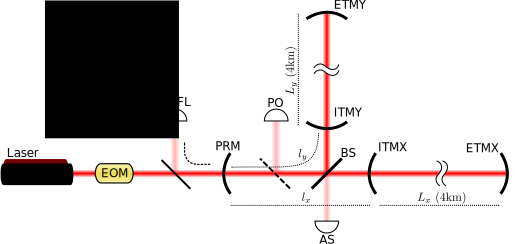
\includegraphics{figs-ifo/prfpmi.pdf}
  \end{center}
  \caption[Diagram of a power-recycled Fabry-Perot Michelson interferometer.]{Diagram of a power-recycled Fabry-Perot Michelson interferometer. \com{more}}
  \label{fig:prfpmi}
\end{figure}
The optical setup of the full LIGO interferometer is quite a bit more complicated than that of a single cavity. %NL%
To maintain the resonance condition of the entire interferometer, it is necessary to sense and control four independent length degrees of freedom. %NL%
It so happens that the technique of PDH reflection locking is well adapted for sensing the length degrees of freedom of more complicated interferometers. %NL%
Placing one's photodetectors at the correct ports of the interferometer can provide all needed information for length sensing. %NL%
The canonical reference on the topic is \citet{Fritschel:01}, but we will provide a short summary.

As seen in Figure \ref{fig:prfpmi}, the interferometer is composed of six primary mirrors. %NL%
Theses are the \emph{power recycling mirror} (PRM), the \emph{beamsplitter} (BS) and the arm cavity optics, refered to as the \emph{end test mass} (ETM) and \emph{input test mass} (ITM), one for each arm, labeled X and Y. %NL%
Only four degrees of freedom are relevent and measurable by their optical path length. %NL%
In the case of LIGO, the degrees of freedom of all the mirrors are measured relative to the ITMs. %NL%
The basis chosen to represent theses lengths is shown in Figure \ref{fig:prfpmi}. %NL%
The length degrees of freedom are refered to as the \emph{differential arm length} (DARM), the \emph{common arm length} (CARM), the \emph{power recycling cavity length} (PRC) and the \emph{Michelson length} (MICH).

Due to the optical topology and location of the sensors, the different sensing ports provide information about the various degrees of freedom of the interferometer. %NL%
As in PDH, the light is phase modulated at RF frequencies before being injected into the interferometer and the length signal is encoded as an RF amplitude modulation of the photodetector power. %NL%
Photodetectors are located at several output ports of the interferometer. %NL%
The modulation can be in the cosine (in-phase, I) or sine (quadrature-phase, Q) quadratures. %NL%
The length degree of freedom with most sensitivity to gravitational waves is DARM, which is the primary signal present at the antisymmetric (AS) port, though the AS port also has some contribution from MICH. %NL%
MICH is the dominant contribution to the power recycling cavity pickoff (PO) port in the Q phase. %NL%
The I phase of the PO port, and the reflection (REFL) port, both have a primary contribution from CARM, with a small contribution from PRC. %NL%
This presents the difficult task of having two sensors which are nearly degenerate in the sensed degree of freedom. %NL%
In LIGO this is solved due to the very high gain of the common mode servo. %NL%
The common mode servo strongly supresses the REFL signal, creating a gain hierarchy with the PO-I signal. %NL%
The signal which remains in PO-I is purely PRC.

The next generation of interferometers, including Advanced LIGO, will include an additional signal recycling mirror which sits between the BS and the AS port. %NL%
This adds an additional length degree of freedom which further complicates the sensing and control \cite{T1000298}.

\section{Non-modulated (DC) readout}
\label{sec:dcreadout}
Prior to the beginning of Advanced LIGO, there was a incremental upgrade called Enhanced LIGO. %NL%
One of the modifications performed during the Enhanced LIGO upgrade was to change the scheme for sensing the DARM degree of freedom. %NL%
The DC power at the AS port has a quadratic dependance on DARM. %NL%
Thus if the arm cavities are differentially detuned slightly (on the order of 10 picometers) from resonance, there will be a linear dependence of the DC power from DARM. %NL%
An alternate picture of the scheme is that in the RF scheme, the RF sidebands are the local oscillator which beats against the gravitational wave sidebands to produce an RF signal, which is a form of heterodyne detection. %NL%
While in the DC case, the DARM offset produces a local oscillator at the same baseband frequency as the signal sidebands, which is a form of homodyne readout. %NL%
A photodetector which measures this DC power is an alternative sensor for reading out DARM. %NL%
DC readout of DARM has been implemented on the GEO600 detector \cite{GEODC}, the Caltech 40 meter prototype interferometer \cite{40mDC}, and for Enhanced LIGO \cite{Tobin}. %NL%
DC readout of DARM is also part of the baseline design for Advanced LIGO. %NL%
A very thorough treatment of the subject can be found in Tobin Fricke's PhD dissertation \cite{FrickeThesis}. %NL%
Here we will cover some of the benefits of such a scheme.

Light which resonates in the compound system composed of the arm cavities and the power recycling cavity experiences an effective cavity bandwidth which is much more narrow than the bandwidth of the arm cavities alone \cite{Rakhmanov}. %NL%
This narrow bandwidth acts as a effective low pass filter of the laser noise fluctuations on the light. %NL%
In the LIGO interferometers, the carrier light is resonant in the coupled cavity system and experiences a filter with a corner frequency of approximately 1Hz. %NL%
The RF sidebands do not resonate in the arm cavities and thus do not experience such dramatic filtering. %NL%
The carrier light thus serves as a much quieter local oscillator than the RF sidebands. %NL%
Thus switching to DC readout can reduce many laser noise couplings.

There is an intrinsic reduction in the shot noise when going from RF to DC readout. %NL%
The total power on the detector is modulated at twice the frequency of the RF sidebands due to the beating of the upper and lower sidebands with eachother. %NL%
The RF demodulation of DARM preferentially samples the signal at the peaks of the RF modulation, leading to a shot noise contribution higher than the DC case by a factor of $\sqrt{3/2}$. %NL%
There is a very nice treatment of this effect in Section 2.9 of Tobin Fricke's dissertation \cite{FrickeThesis}.

One of the drawbacks of DC readout is that the audio modulation of any of the optical fields present at the AS port can cause noise in the readout. %NL%
To mitigate the existence of the fields not necessary for producing the signal, i.e. %NL%
any fields that are not the local oscillator or the signal fields, one may utilize an output mode cleaner. %NL%
The output mode cleaner acts as both a spatial and frequency filter of the fields detected at the AS port and will be described in detail in the following chapter.
